\section{Thermal mass estimation}
\label{ch:thermtool}
Decelerating an entry vehicle requires a thermal protection system. This system will contribute to a large extend to the mass of the entire vehicle. Therefore, a thermal protection system (\gls{tps}) has a critical impact on the mission an should be selected properly. This section will analyse the \gls{tps} of the five trade-off concepts with the use of a thermal protection tool. First the tool will be described in more detail. Afterwards it is described how the tool is verified and validated. In the third section, this tool will be used to analyse different lay-ups for the concepts under anlysis. As a result,the \gls{tps} masses for differnt concepts can be determined. Lastly, concluions and recomendations.\\

\subsection{Method of thermal analysis}
A mass estimations of the \gls{tps} requires analysis due to heat transfer in the heat shield. Enable to analyse different lay-ups in a short amount of time, it will be usefull to make use of a \gls{tps} tool. The working principles of this tool are describes in detail in this section.\\

\subsubsection{Assumptions}
In this section the assumptions that are used for the \gls{tps} mass estimation and tool developement are stated. Also, an elaboration is given of the impact of the assumption on the results.\\

\begin{itemize}
\item \textbf{1D instead of 3D analysis}: For the determination of the temperature through the material over time, a one dimensional lay-up can be used. This is different from the actual case, where the body is heated over a three dimentional body. This assumption however is varied for instance by Ref. \cite{Corso2009}.
\item \textbf{Sizing is done under stagnation conditions}: One of the inputs in the tool is the temperature at the wall. For this, the stagnation temperature is used instead of the actual temperature distribution over the surface. The stagnation temperature is a maximum value for the temperature and hence, the result of the tool will give the most conservative value needed for the design of the \gls{tps}. Therefore, the \gls{tps} will be overdesigned and can not be used as final values of the \gls{tps} mass. However, they do give an indication on how different concepts perform relative to eachother, such that the method can be used to make trade-off desisions.
\item \textbf{Model for heat flux}: Another input in the tool is the heat flux. This heatflux input is based on an aerodnamic model described, as described in Chapter \ref{ch:aero_analysis}.
\item \textbf{Constant material properties}: Material properties like tensile stregth, density and thermal conductivity change, if considered over a large temperature range. However, it is assumed that this change is negligable. 
\item Ablative materials of rigid structures are assumed not to reduce in thickness as a first approximation.
\item \textbf{Appliable to multiple layers}: The tool uses steps in legth that pass over layers with different materials. It is possible that a length step is located inbetween two layers but is only concidered as one material. Because length steps are very small, this has no major impact on the model.
\item \textbf{discritisation of differential equations}: The tool is based on a finite difference discritisation. This method is verified. However, the discritisation errors are only stable for a certain range of time steps, as can be seen in Ref. \cite{Smith2011}. 
\end{itemize}

\subsubsection{Leading equations}
The problem is modelled as a one-dimensional multilayer layup which can provide the accuracy needed or this stage of concept analysis as described in the assumptions. A description of the implementation of this model is given by Smith \cite{Smith2011}. The model is illustrated in Figure \ref{fig:1dthermal}. The figure shows the different methods of heat transfer in the model. There is heat radiating away from the surface, convective heating or heat flux from the aerodynamic effects and heat conduction within the layers.

\begin{figure}[H]
	\centering
	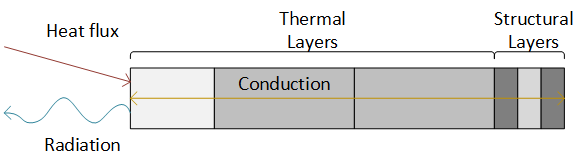
\includegraphics{Figure/1dthermal.png}
	\caption{1D thermal model}
	\label{fig:1dthermal}
\end{figure}

The layup is then discretised in $i_{max}$ nodes, each having a thickness of $\Delta \gls{sym:x}$. For the nodes that only experience conduction as heat transfer the one-dimensional, time-dependent (transient) heat equation can be used, which is given by Equation \eqref{eq:therm1}

\begin{equation}
\frac{\partial \gls{sym:T}}{\partial \gls{sym:t}} = \gls{sym:alphat}\frac{\partial^2\gls{sym:T}}{\partial \gls{sym:x}^2}
\label{eq:therm1}
\end{equation}

In this equation $\gls{sym:alphat}=\frac{\gls{sym:k}}{\rho \gls{sym:cp}}$ stands for the thermal diffusivity, \gls{sym:k} for the thermal conductivity, $\rho$ the material density and \gls{sym:cp} the material specific heat. Since the layup has been discretised, the heat equation is discretised as well. The time march method used for this discretisation is the Forward in Time and Central in Space (FTCS) scheme is used. The advantage of this time march is that it is computationally inexpensive. The drawback is that it can be unstable and therefore $\Delta \gls{sym:t}$ and $\Delta \gls{sym:x}$ should be chosen such that it complies with a stability criterion. The result of the time march is given by Equation \eqref{eq:therm2}. The notation in the equation is as follows: the subscript $i$ refers to the node and the superscript $n$ refers to the timestep. Obviously, the distance between $i$ and $i+1$ is $\Delta \gls{sym:x}$ and the time between $n$ and $n+1$ is $\Delta \gls{sym:t}$.

\begin{equation}
\frac{\gls{sym:T}_i^{n+1}-\gls{sym:T}_i^n}{\Delta \gls{sym:t}} = \gls{sym:alphat}\left[\frac{\gls{sym:T}_{i+1}^n-2\gls{sym:T}_i^n+\gls{sym:T}_{i-1}^n}{\left(\Delta \gls{sym:x}\right)^2}\right]
\label{eq:therm2}
\end{equation}

This equation can be rewritten such that it shows the heat rate balance of a node per unit area in $\left[\frac{W}{m^2}\right]$ (Equation \eqref{eq:therm3}). This can be done by writing out \gls{sym:alphat}. To account for different materials in the layup, the heat transfer between the neighbouring nodes is separated. For this the factors $\gls{sym:K}_{i-1}=2\left(\frac{1}{\gls{sym:k}_{i-1}}+\frac{1}{\gls{sym:k}_i}\right)^{-1}$ and $\gls{sym:K}_{i+1}=2\left(\frac{1}{\gls{sym:k}_{i+1}}+\frac{1}{\gls{sym:k}_i}\right)^{-1}$ are used. The same behaviour can be seen in electrical resistance as the inverse of the equivalent resistance is the sum of the inverse resistances in a parallel circuit ($\frac{1}{R_{eq}}=\frac{1}{R_1}+\frac{1}{R_2}$). This heat rate balance can also be presented schematically as shown in Figure \ref{fig:thermbalance1}.

\begin{equation}
\frac{\rho_i\gls{sym:cp}_i\Delta \gls{sym:x}}{\Delta \gls{sym:t}}\left(\gls{sym:T}_i^{n+1}-\gls{sym:T}_i^n\right)=\frac{\gls{sym:K}_{i-1}}{\Delta \gls{sym:x}}\left(\gls{sym:T}_{i-1}^n-\gls{sym:T}_i^n\right)-\frac{\gls{sym:K}_{i+1}}{\Delta \gls{sym:x}}\left(\gls{sym:T}_i^n-\gls{sym:T}_{i+1}^n\right)
\label{eq:therm3}
\end{equation}

\begin{figure}[H]
	\centering
	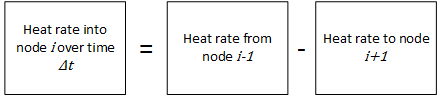
\includegraphics{Figure/thermblocknode1.png}
	\caption{Heat rate balance for conducting nodes}
	\label{fig:thermbalance1}
\end{figure}

Recall that the first node, or the surface node also experiences radiation and convection. The heat rate balance can be easily illustrated by changing the blocks in the previous scheme according to the aforementioned differences. The surface node receives the heat flux, radiates heat away and conducts heat to node $i+1$ (or node 2). No conducted heat is received from node $i-1$ since node 0 does not exist. These changes result in Figure \ref{fig:thermbalance2}.

\begin{figure}[H]
	\centering
	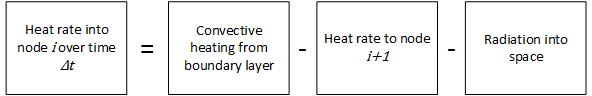
\includegraphics{Figure/thermblocknode2.png}
	\caption{Heat rate balance for conducting nodes}
	\label{fig:thermbalance2}
\end{figure}

Equation \eqref{eq:therm3} can then be altered by adding a $q^n$-term for the convective heating, or heat flux and adding  $\gls{sym:eps}\gls{con:stefanboltzmann}\left(\left(\gls{sym:T}_1^4\right)^n-\left(\gls{sym:T}_\infty^4\right)^n\right)$ to account for the radiation. In here the superscript $n$ stands for timestep $n$. For the last node a similar heat balance can be constructed. Smith says that in this node the radiation and convection terms can omitted since they are much lower than the conductive heat rate in this part \cite{Smith2011}. In this case all heat conducted from node $i-1$ is stored into node $i$ as conduction towards node $i+1$ is not possible.


\subsubsection{Input}
In order to make use of the tool, an input is required. This input consist of thermal conditions and material properties for five different concepts. The thermal properties are the stagnation temperature $ \gls{sym:T0}(t) $ and a stagnation heat flux $ \gls{sym:qsdot}(t) $. The material properties are the layer thickness $ L_1 $, $ L_2 $, etc., The thermal conducticity $ \gls{sym:k} $, the density $ \gls{sym:rho} $ and lastly the specific heat $ \gls{sym:cp} $.\\

Thermal inputs for the five condepts, temp and flux + graph.\\

Several lay-ups are analysed, all with a variety of materials. An overview of these materials with their properties is shown in Table \ref{tab:tpsmatprop}.

\begin{table}[H]
\caption {TPS Material properties}
\centering
    \begin{tabular}{|l|l|l|l|l|}
    \hline
    \textbf{Material}         & \textbf{Conductivity $ \frac{W}{m*K} $} & \textbf{Density $ \frac{kg}{m^3} $} & \textbf{Specific heat \ $ \frac{J}{kg*K} $ }& \textbf{Emissivity $  [ - ] $} \\ \hline \hline
    Nextel AF14       & 0.150                                                 & 858                                        & 1050                                            & 0.443                                      \\ \hline
    Nextel BF20       & 0.146                                                 & 1362                                       & 1130                                            & 0.443                                      \\ \hline
    Nextel XN513      & 0.148                                                 & 1151                                       & 1090                                            & 0.443                                      \\ \hline
    Refrasil C1554-48 & 0.865                                                 & 924                                        & 1172                                            & 0.7                                        \\ \hline
    Refrasil UC100-28 & 0.865                                                 & 890                                        & 1172                                            & 0.2                                        \\ \hline
    Hexcel 282 Carbon & 0.5                                                   & 891                                        & 1000                                            & 0.9                                        \\ \hline
    Pyrogel 6650      & 0.030                                                 & 110                                        & 1046                                            & ~                                          \\ \hline
    Pyrogel 5401      & 0.0248                                                & 170                                        & 1046                                            & ~                                          \\ \hline
    Pyrogel 1800      & 0.085                                                 & 156                                        & 1172                                            & ~                                          \\ \hline
    Pyrogel 2000      & 0.095                                                 & 180                                        & 1172                                            & ~                                          \\ \hline
    KFA 5             & 0.25                                                  & 98                                         & 1250                                            & ~                                          \\ \hline
    Kapton            & 0.12                                                  & 1468                                       & 1022                                            & ~                                          \\ \hline
    Upilex            & 0.29                                                  & 1470                                       & 1130                                            & ~                                          \\ \hline
    \end{tabular}
    \label{tab:tpsmatprop}
\end{table}

\subsubsection{Output}


\subsection{Verification \& Validation}

\subsubsection{Verification}
Suthes
\subsubsection{Validation}



\subsection{Results per concept}



\subsection{Conclusion \& recomendations}
Check for material failure other then for thermal reasons.
